\subsection{Gestion de la carte}

Le modele du MVC permet de stocker toutes les données de la simulation. Un carte est un tableau en deux dimensions de taille fixe qui contient des éléments de type Content. Ainsi au démarrage de l'application le modele est initialisé en parsant le fichier de carte sur lequel on veut jouer. Les données lues au moment du parsing sont stockées dans un objet de type Board dont voici la description : \\[0.5cm]
\centerline{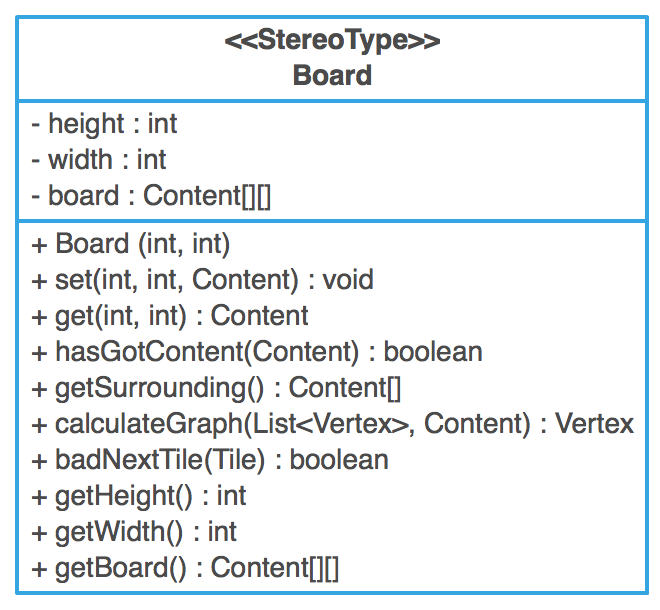
\includegraphics[scale=0.2]{Map}}

Le choix du tableau de taille fixe nous permet d'autre part de gérer les fichiers malformés, les dépassement ce tableau... En effet, c'est grâce à cette objet que nous pouvons tester les cartes "pourries" (les cartes où Pacman ne pourra jamais gagner car il est bloqué).
